% ==============================================================================
% PG - Israel dos Santos Candeias
% Capítulo 2 - Referencial Teórico
% ==============================================================================
\chapter{Referencial Teórico e Tecnologias Utilizadas}
\label{sec-referencial}
% Este capítulo deve apresentar os aspectos relativos ao conteúdo teórico relevante para o trabalho.  Incluirá conhecimento adquirido a partir de livros, artigos, relatórios técnicos, dissertações, teses e outros materiais bibliográficos.  O capítulo deve apresentar, além do referencial teórico, informações sobre as tecnologias utilizadas no trabalho. O capítulo deve ter cerca de 12-15 páginas e deve demonstrar conhecimento básico da literatura técnico-científica sobre o tema abordado no trabalho.
Neste capítulo serão apresentados os conceitos teóricos que guiaram o desenvolvi
mento do jogo, bem como as tecnologias usadas para implementar o sistema
% colocar os links para as seções explicando oq cada uma fala 

\section{Princípios de Design de Software}
Os princípios de design de software constituem diretrizes fundamentais para o desenvolvimento de sistemas de software eficazes, robustos e manuteníveis. Esses princípios orientam todo o ciclo de vida do software desde o surgimento da ideia até o sistema em produção. 
\subsection{Engenharia de Software}
A engenharia de sofware é a área da computação que se preocupa em propor e aplicar princípios de engenharia na construção de softwares\cite{EngSoftMod} ou seja é uma área de estudos da computação que se preocupa em projetar, arquitetar melhorar a qualidade dos produtos de software e aumentar a produtividade no processo de desenvolvimento. 

Para seguir as práticas recomendadas de engenharia de software o primeiro passo a ser definido é qual paradigmas de processo de software ser seguido, existem vários modelos para diferentes cenários possíveis, o escolhido para esse trabalho foi o modelo evolutivo.

O modelo evolutivo como seu nome sugere, os requisitos vão evoluindo conforme a aplicação evolui, esse processo ocorre em paralelo à evolução da aplicação, esse paradigma é muito útil quando o cliente não tem todas as funcionalidades necessárias para a solução. Nesse contexto foi oque mais se adequou a esse trabalho tendo em vista que nem todos os requisitos eram bem definidos de início e as funcionalidades do jogo precisam ser validadas frequentemente, uma vez que, a jogabilidade precisa ser atraente ao público, então a cada nova versão foram realizadas reuniões com colegas, e com a orientadora, a fim de receber feedbacks que auxiliem na melhoria dos recursos de modo contínuo.

\newpage
\begin{figure}
    \centering
    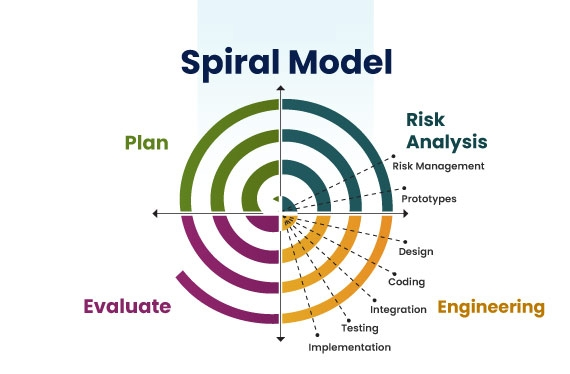
\includegraphics[width=0.9\linewidth]{figuras/spiral_model.jpg}
    \caption{Ciclo de vida do modelo espiral}
    \label{fig:enter-label}
\end{figure}
Cada uma das atividades realizadas no modelo ilustrado acima são:
\begin{itemize}
    \item \textbf{Planejamento:} A fase de planejamento é base sobre a qual todo o projeto de desenvolvimento de software deve ser construído. Durante essa fase foram definidos os requisitos e as ferramentas que seriam utilizadas;
    \item \textbf{Análise de riscos:} Nessa fase é feito tanto o levantamento dos riscos associados ao desenvolvimento do sistema, mas também como mitigá-los no geral sendo uma etapa para gerenciar os riscos, e na avaliação da viabilidade técnica. 
    \item \textbf{Engenharia (Projeto e Codificação):} Aqui é onde são desenvolvidos os o designs do software, codificação, integração, testes e por fim a implantação no sistema.
    \item \textbf{Validação):} Ao chegar nessa fase já temos uma versão 1.0 e podemos coletar feedbacks o observações sobre o sistema, essa etapa é fundamental nessa abordagem, pois a qualidade da próxima versão é diretamente proporcional a qualidade dos feedbacks aqui coletados.
\end{itemize}
\section{Pygame-ce}
Pygame-ce (Community Edition) é uma biblioteca multiplataforma gratuita e de código aberto que surgiu de um fork do projeto pygame por seus antigos desenvolvedores principais, e foi criado após desafios impossíveis os impedirem de continuar o desenvolvimento upstream. Essa nova distribuição visa oferecer lançamentos mais frequentes, correções de bugs e melhorias contínuas para o desenvolvimento de aplicativos multimídia como videogames utilizando a linguagem Python. Ela usa a biblioteca SDL (Simple DirectMedia Layer)\footnote{SDL (Simple DirectMedia Layer) \url{https://www.libsdl.org/}} que é uma biblioteca de desenvolvimento multiplataforma projetada para fornecer acesso de baixo nível a hardware de áudio, teclado, mouse, joystick e gráficos via OpenGL e Direct3D além de várias outras bibliotecas populares para abstrair as funções mais comuns, tornando a escrita desses programas uma tarefa mais intuitiva, assim então permitindo que você crie jogos e programas multimídia com todos os recursos na linguagem python.\cite{Pygame-ce}

As principais funcionalidades do pygame incluem
\begin{itemize}
    \item carregar e exibir imagens;
    \item criar animações e renderizar quadros de jogos;
    \item adicionar música de fundo e efeitos sonoros;
    \item Manipulação de dispositivos de entrada;
    \item Gerenciamento de sprites através de classes integradas;
\end{itemize}

Como a maioria das bibliotecas no python ela pode ser adicionada via prompt de comandos do sistema operacional  por meio do pip\footnote{pip \url{https://pip.pypa.io/en/stable/}}, o pip é um sistema de gerenciamento de pacotes para Python, usado para instalar e gerenciar pacotes de software escritos na linguagem de programação Python. Ele simplifica o processo de instalação, atualização e remoção de pacotes Python e suas dependências. 
% colocar em código
% colocar um codigo com \href{https://pyga.me/docs/ref/music.html}{pygame.mixer.música} \href{https://pyga.me/docs/ref/draw.html}{pygame.draw} 
% \href{https://pyga.me/docs/ref/event.html}{pygame.event} 
% \href{https://pyga.me/docs/ref/font.html}{pygame.font} 
% \href{https://pyga.me/docs/ref/image.html}{pygame.image} 
% \href{https://pyga.me/docs/ref/key.html}{pygame.key} 
% \href{https://pyga.me/docs/ref/rect.html}{pygame.Rect} 
% \href{https://pyga.me/docs/ref/sprite.html}{pygame.sprite} 
% \href{https://pyga.me/docs/ref/surface.html}{pygame.Surface} 
% \href{https://pyga.me/docs/ref/transform.html}{pygame.transform} 
% \href{https://pyga.me/docs/ref/window.html}{pygame.Window} 
Após isso ja é possível acessar e usar a biblioteca por meio do "import" do python como no exemplo abaixo que demonstra uma main de projeto pygame.


\newpage
\begin{lstlisting}[language=C++,breaklines, caption= Instalação Pytmx]
pip install pygame-ce
\end{lstlisting}

\begin{lstlisting}[language=Python,breaklines, caption= Exemplo de main de um projeto Pygame]
# Arquivo de exemplo mostrando um "game loop" básico do pygame
import pygame

# pygame setup
pygame.init() 
screen = pygame.display.set_mode((1280, 720))
clock = pygame.time.Clock()
running = True

while running:
    # poll for events
    # pygame.QUIT event means the user clicked X to close your window
    for event in pygame.event.get():
        if event.type == pygame.QUIT:
            running = False

    # fill the screen with a color to wipe away anything from last frame
    screen.fill("purple")

    # RENDER YOUR GAME HERE

    # flip() the display to put your work on screen
    pygame.display.flip()

    clock.tick(60)  # limits FPS to 60

pygame.quit()
\end{lstlisting}
Esse é um exemplo básico de uma main  com uma configuração básica, na linha (2) importamos o pygame e dizemos ao compilador 


\section{Pytmx}
PyTMX é um carregador de mapas para python/pygame projetado para jogos. Ele fornece carregamento inteligente de tiles com uma base de armazenamento rápida e eficiente. Ele não apenas manipula corretamente a maioria dos tipos de objetos Tiled, como também carrega metadados para eles, para que você possa modificar seus mapas e objetos no Tiled, em vez de modificar seu código-fonte.\cite{PyTMX} 
Pytmx também é uma biblioteca e pode ser instalada por via de comando com o pip 
\begin{lstlisting}[language=C++,breaklines, caption= Instalacao Pytmx]
pip install pytmx
\end{lstlisting}

este é um exemplo básico de utilização da biblioteca onde estamos carregando o map.tmx para dentro do python
\begin{lstlisting}[language=C++,breaklines, caption= utilização básica Pytmx]
from pytmx.util_pygame import load_pygame
tmxdata = load_pygame("map.tmx")
\end{lstlisting}

\section{\textbf{Propriedades de Tile, Object e Map}}

Propriedades são um recurso poderoso do Tiled que permite ao designer de níveis atribuir dados de chave/valor a mapas, tilesets, tiles e objetos individuais. O Pytmx inclui suporte completo para leitura desses dados para que você possa definir parâmetros para coisas no Tiled, em vez de manter arquivos de dados externos, ou mesmo valores na fonte.

Propriedades de blocos individuais são acessadas por meio do objeto de mapa pai:
% >>> tmxdata = TiledMap('level1.tmx')
% >>> props = txmdata.get_tile_properties(x, y, layer)
% >>> props = tmxdata.get_tile_properties_by_gid(tile_gid)
 

\section{Editor de mapas}
citar jogos populares que utilizam essa tecnica (dofus)
% explicar oq e um editor de mapas
\subsection{Tile}
Tile (Azulejo) 
Tileset é um Um conjunto de azulejos é um recurso gráfico para desenhar níveis e outros componentes estáticos do seu jogo. Um tile set é composto de uma única imagem que é então dividida em diferentes "células" (tiles), e cada tile pode então ser colocado no editor room para criar uma imagem completa. Abaixo você pode ver dois exemplos sprites que podem ser usados como conjuntos de azulejos:
\subsection{Tiled}
% explicar o uq é um tile

% resumir tudo isso
Tiled é um editor de níveis 2D que ajuda você a desenvolver o conteúdo do seu jogo. Seu recurso principal é editar mapas de tiles de várias formas, mas ele também suporta posicionamento de imagem livre, bem como maneiras poderosas de anotar seu nível com informações extras usadas pelo jogo. Tiled foca na flexibilidade geral enquanto tenta permanecer intuitivo.

Em termos de mapas de tiles, ele suporta camadas de tiles retangulares retas, mas também camadas isométricas projetadas, isométricas escalonadas e hexagonais escalonadas. Um tileset pode ser uma única imagem contendo muitos tiles ou pode ser uma coleção de imagens individuais. Para suportar certas técnicas de simulação de profundidade, tiles e camadas podem ser deslocados por uma distância personalizada e sua ordem de renderização pode ser configurada.

O Tiled também suporta camadas de objetos , que tradicionalmente eram apenas para anotar seu mapa com informações, mas mais recentemente também podem ser usadas para colocar imagens. Você pode adicionar objetos retângulos, pontos, elipses, polígonos, polilinhas e ladrilhos. O posicionamento de objetos não se limita à grade de ladrilhos e os objetos também podem ser dimensionados ou girados. As camadas de objetos oferecem muita flexibilidade para adicionar quase qualquer informação ao seu nível que seu jogo precise.

\section{Pixel Art}
Pixel é a menor unidade de uma imagem e se você fizer uma aproximação de uma foto digital ou de uma tela de celular, verá uma série de quadradinhos. Cada um deles é um pixel.
Pixel Art é um tipo de arte que usa pixels visíveis para compor uma imagem ou um vídeo
% explicar oq é pixel art
\subsection{Aseprite}
% Para fazer um jogo é necessário ter sprites 
O Aseprite é uma ferramenta que permite que você crie animações 2D para videogames. De sprites a pixel-art, gráficos estilo retrô e tudo o que você gosta sobre a era de 8 bits e 16 bits . \cite{Aseprite}

No Aseprite, um sprite consiste em uma sequência de quadros e uma pilha de camadas. A intersecção de quadros e camadas cria uma matriz de células gráficas editáveis com imagens/pixels que podem ser editados com o editor de sprites . Camadas, quadros e células são visíveis na linha do tempo :

Um quadro é uma única imagem estática em um sprite. Adicionar e alterar quadros cria uma sequência de imagens chamada animação